A \emph{concept} in the CML metamodel is used to represent anything
that has a coherent, cohesive meaning in a domain.
On the ER \cite{er} metamodel,
it corresponds to an \emph{entity};
on the UML \cite{uml} metamodel,
to a \emph{class}.
The CML \emph{concept} differs, however, from the UML \emph{class},
because it contains only \emph{properties},
while the UML \emph{class} may also have \emph{operations}.

Figure \ref{fig:ex:concepts} presents some examples of \emph{concepts} declared in CML.
As shown in the examples,
a \emph{concept} may have zero or more \emph{properties}
(\ref{sec:properties}),
and a \emph{property} may optionally declare a \emph{type}
(\ref{sec:primitive-types}, \ref{sec:collection-types}).
Also, as shown in the last example of figure \ref{fig:ex:concepts},
a \emph{concept} may specialize
(\ref{sec:generalization})
another \emph{concept}.

\begin{figure}
\verbatimfont{\small}
\begin{framed}
\verbatiminput{examples/concepts.cml}
\end{framed}
\caption{Concept Examples}
\label{fig:ex:concepts}
\end{figure}

Figure \ref{fig:stx:concept} specifies the syntax used
to declare a \emph{concept}.
The \textbf{concept} keyword is followed by a NAME.
Optionally, a list of other NAMEs may be enumerated,
referring to other \emph{concepts}
that are generalizations (\ref{sec:generalization}) of the declared \emph{concept}.
Under the \textbf{concept} block,
a list of \emph{properties} (\ref{sec:properties}) may be declared as well.
The \textbf{abstract} keyword may precede the \textbf{concept} keyword, making a \emph{concept} abstract (\ref{sec:abstract}).

\begin{figure}
\verbatimfont{\small}
\begin{framed}
\verbatiminput{grammar/Concepts.txt}
\end{framed}
\caption{Concept Declaration Syntax}
\label{fig:stx:concept}
\end{figure}

\begin{figure}
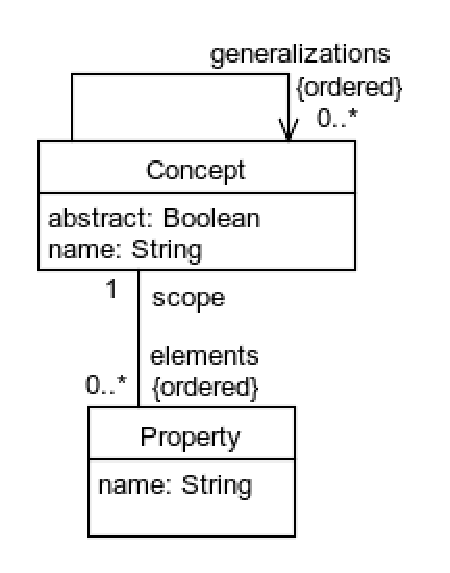
\includegraphics[width=\textwidth]{metamodel/concept}
\caption{Concept Metamodel}
\label{fig:stx:concept}
\end{figure}
